\documentclass[
	english,
	fontsize=10pt,
	parskip=half,
	titlepage=true,
	DIV=12
]{scrartcl}

\usepackage[utf8]{inputenc}
\usepackage{babel}
\usepackage[T1]	{fontenc}
\usepackage{lmodern}
\usepackage{microtype}
\usepackage{color}
\usepackage{csquotes}

\usepackage{hyperref}

\usepackage{graphicx}
\usepackage{wrapfig}
\usepackage[bf]{caption}
	\captionsetup{format=plain}

\newcommand*{\tabcrlf}{\\ \hline}

\usepackage{amsmath}

\usepackage{minted}
	\usemintedstyle{friendly}

\newcommand*{\inPy}[1]{\mintinline{python3}{#1}}
\newcommand*{\ie}{i.\;e. }
\newcommand*{\eg}{e.\;g. }

\newcommand{\thus}{\ensuremath{\rightarrow}}

\begin{document}

\part*{Python Problems 12, Winter 2021/22}
\section{Bakeries (2\;P)}
Let's imagine you want to open a bakery shop. As an avid entrepreneur you first analyze your competitors: for all other bakeries in town, you find out what they sell, how much fat and sugar their products contain, how much of them they sell and how much money they make on these products. With these data you want to decide whether healthier (low-sugar, low-fat) products perform better than high-calorie ones, and which price regime is apt for what products. To that end, you want to visualize the data you've collected as a scatterplot.

On GRIPS, you'll find the file elections.csv\footnote{which was created by using the script analyze\_bakeries.py. You can download it from GRIPS, too, if you're curious}. Read the data into memory, and create a plot from them. For each product sold in town, there should be a dot on your chart. The position on the chart should be given by the fat and sugar content. For the size, use the information how often the product is sold. Use the price to colour the dots. Don't forget to put labels on the axes and a title on top of the figure.

\emph{Hint:}\\
To insert a colorbar with label, use the line:
\mint{python3}{plt.colorbar().set_title("foo bar")}

You don't have to add a label for the sizes of your dots.


\section{German Elections (2\;P)}
On GRIPS, you'll find the file elections.csv\footnote{which was with the data you can find on \url{https://www.bundestag.de/parlament/wahlen/ergebnisse_seit1949-244692}}. It contains the results of the federal elections in Germany for the years 1949--2021. From these, generate the following plot:

\begin{center}
	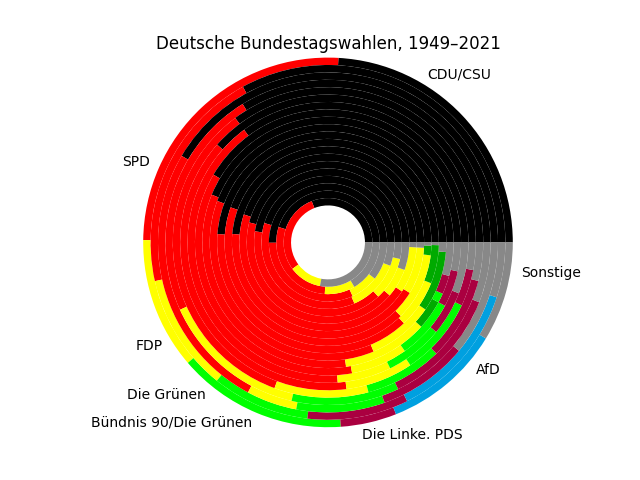
\includegraphics[width=.7\linewidth]{./elections}
\end{center}

\emph{Hint:}\\
To create nested pie plots, you can use the optional parameter \texttt{radius}. It can take a float value that represents the radius of the pie chart to plot. Further, the optional parameter \texttt{wedgeprops} controls further details about how the slices of the pie chart are rendered on screen. It takes a \inPy{dict} that maps certain strings to numeric values. One of these strings is \inPy{'width'}, which tells the matplotlib how wide a ring in the pie chart should be. I used a width of 0.05.


\section{Predator/Prey: Lotka–Volterra Model (3\;P)}
We want to simulate and visualize the extent of a population of two species of animals. One of them will be the prey of the other species, so we might be dealing with rabbits and wolves.

We assume that, for the prey species, ressources are nigh-unlimited, so they'll undergo exponential growth: in each time step (\eg in each year) they grow by a given factor $1 + \alpha$. (Think of $\alpha$ as the percentage of growth. $\alpha = 1$ means 100\% growth rate or doubling of the population each year.)

\emph{Example:}\\
In the first year, there are 100 rabbits. $\alpha = 1$. Then, in the second year, there are 200 rabbits, in the third year there are 400 rabbits, in the fourth year 800 rabbits, and so on.

However, there also are predators which hunt and kill the prey species. The more predators there are, the more difficult it gets for the prey, and the more prey animals there are the easier the predators find lunch. The number of killed prey animals is given by $\beta \times \text{[number of prey animals]} \times \text{[number of predator animals]}$, where $\beta$ is some number constant.

\emph{Example:}\\
In the first year, there are $x = 100$ rabbits and $y = 2$ wolves. $\alpha = 1$ and $\beta = 0.25$. Then, the change $\Delta x$ in the rabbit population is:
\[ \Delta x = \alpha x - \beta x y = 1 \times 100 - 0.25 \times 100 \times 2 = 50 \]
So, one year later, there are 50 more rabbits and a total of 150 rabbits.

The predators grow proportionally to the number of prey animals they kill. Also, each year, a fixed portion of them die of old age. Hence, there will be proportionality constants $\gamma$ and $\delta$ that tell you how many predators are born and die each year.

\emph{Example:}\\
In the first year, there are $x = 100$ rabbits and $y = 2$ wolves. $\gamma = 0.1$ and $\delta = 0.5$. Then the change $\Delta y$ in the wolf population is:
\[ \Delta y = \gamma x y - \delta y = 0.1 \times 100 \times 2 - 0.5 \times 2 = 19 \]
So in the second year, there will be 19 more wolves and a total of 21 wolves.

As a last refinement, we should not forget, that not all prey- and predator animals are born at the same time, nor do they die in sync. To reflect that fact, we evaluate the model several times per year and re-scale the effects on the predator- and prey-populations by the number of times we evaluate.

\emph{Example:}\\
We compute the number of rabbits and wolves each month, i.e. $T = 12$ times per year. With this, we get for the first month:
\begin{align*}
	\Delta x_1 &= \frac{1}{T} (\alpha x   - \beta x y) = \frac{50}{12} \\
	\Delta y_1 &= \frac{1}{T} (\gamma x y - \delta  y) = \frac{19}{12}
\end{align*}
which gives 104.16 rabbits and 3.58 wolves after the first month. (Ignore the fact that this gives you non-integer numbers here.) For the second month, you plug back $x = 104.16$ and $y = 3.58$ into the equation, and so forth.

Implement this model and show the evolution of the animals in a plot. I used the parameters $x_0 = 10, y_0 = 5, \alpha = 1.0, \beta = 0.3, \gamma = 0.1, \delta = 0.3, \frac{1}{T} = 0.0001$ to obtain this graph:

\begin{center}
	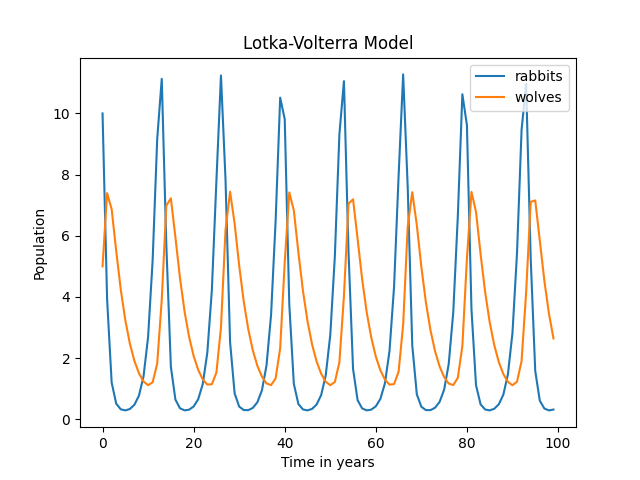
\includegraphics[width=.6\linewidth]{./Lotka-Voltera}
\end{center}

\end{document}
